\qquad A análise de complexidade do Insertion Sort, considerando as
diferentes situações de entrada (crescente, decrescente e
randômica), foi realizada manuscrita, com a devida justificativa,
contando o número de execuções de cada linha do algoritmo (associando
uma constante de custo $c_i$ a cada linha) e somando essas contagens
em função de $n$, conforme exigido pelo enunciado do trabalho.

\begin{figure}[htbp]
    \centering
    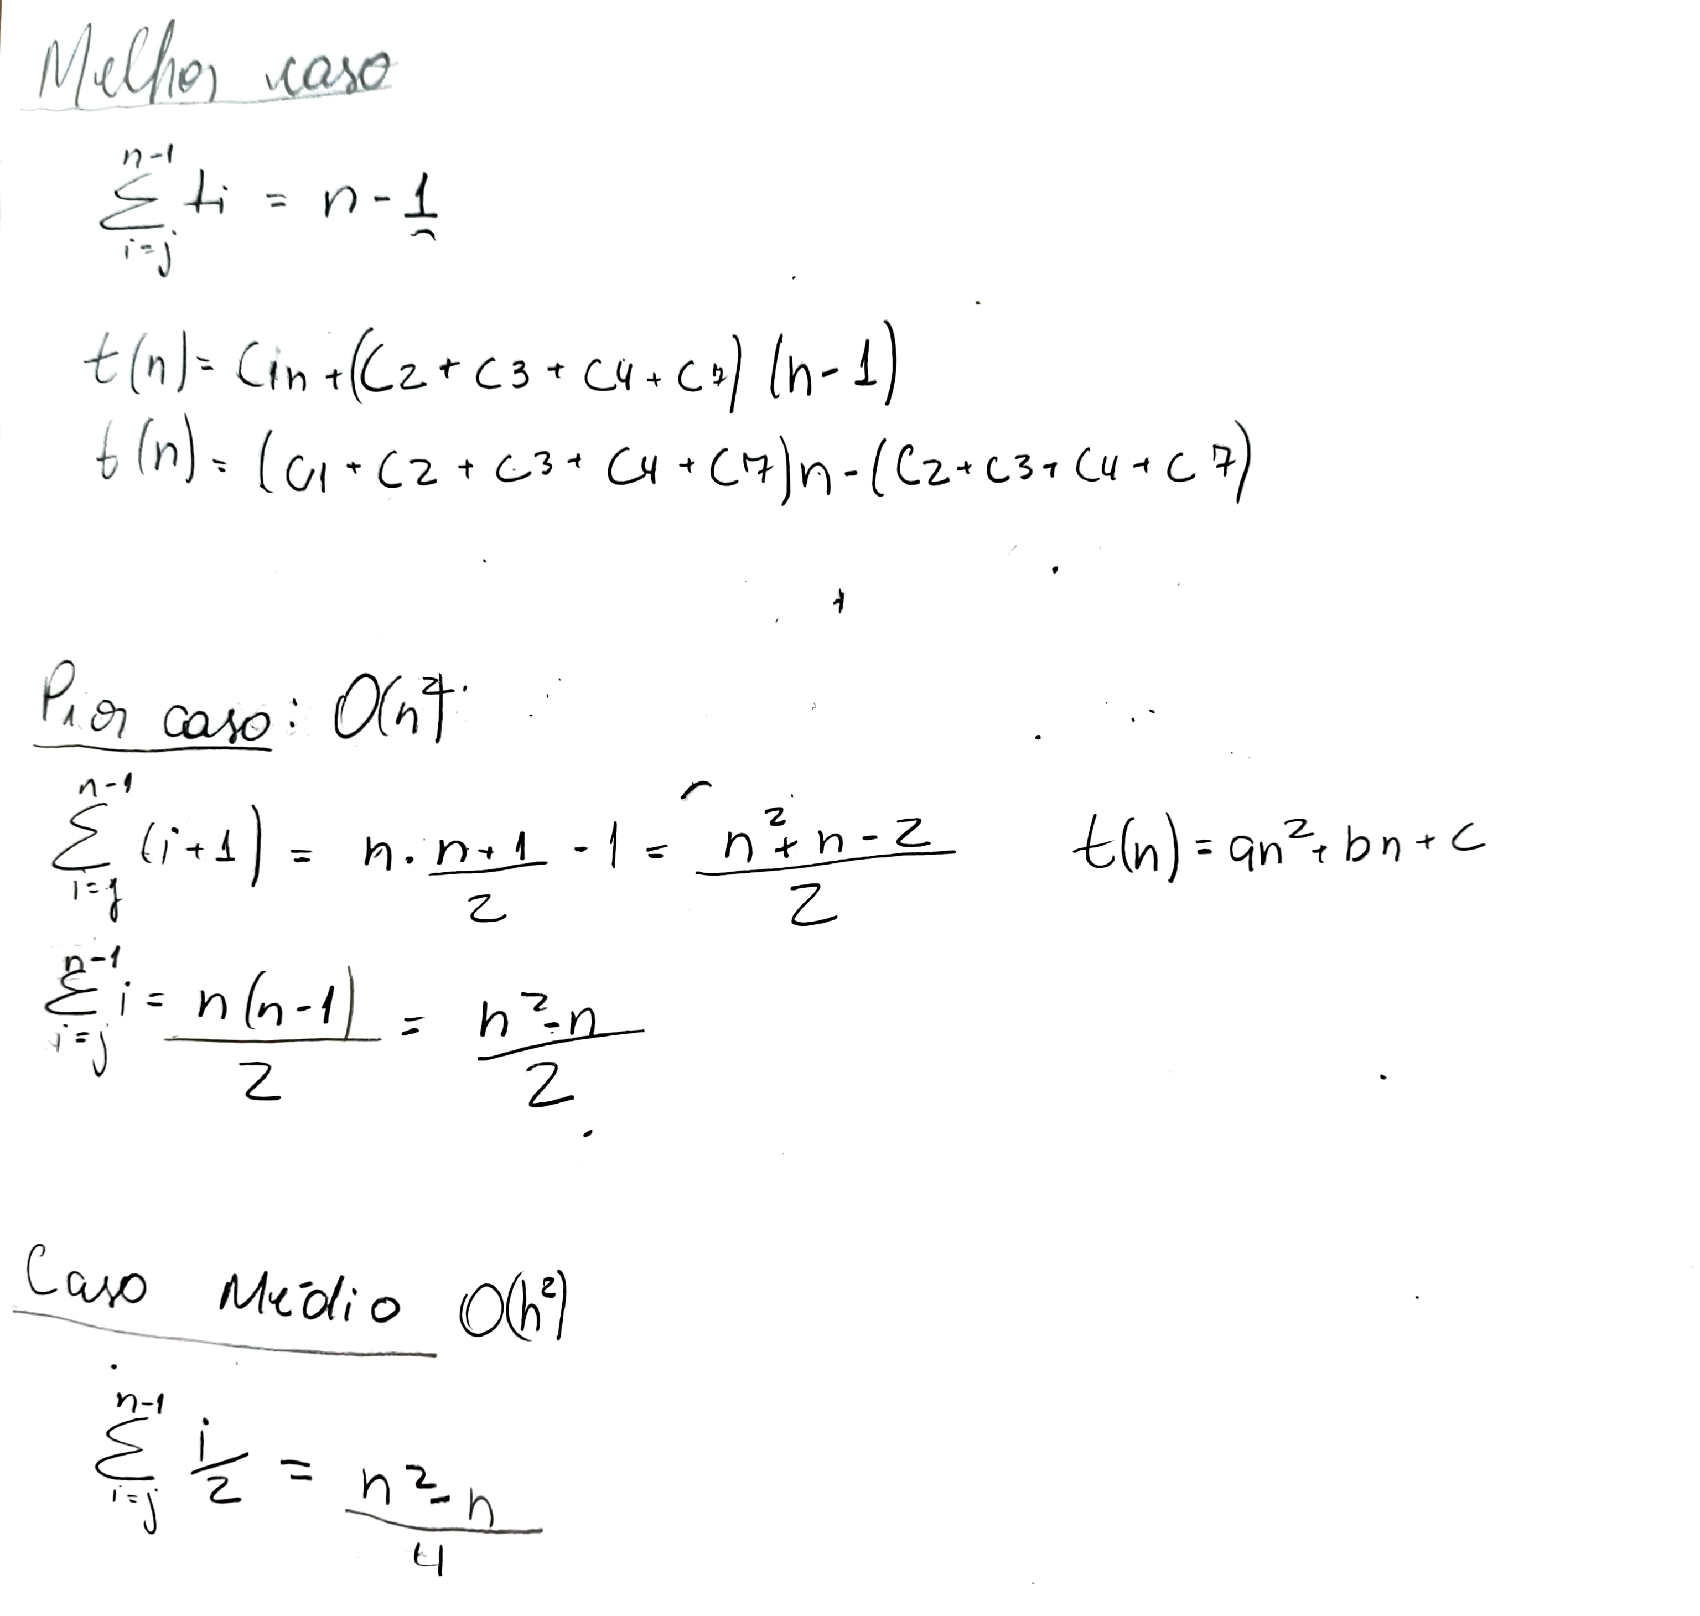
\includegraphics[width=14cm]{Imagens/Insertion Sort/analise_complexidade.png}
    \caption{Análise de complexidade manuscrita do algoritmo Insertion Sort}
    \label{fig:analise_complexidade}
\end{figure}

\qquad Em resumo, a análise manuscrita chega às seguintes conclusões
para cada situação de entrada:

\textbf{Melhor caso (entrada crescente):} o laço interno nunca
desloca elementos, pois cada elemento já está na posição correta.
A contagem resulta em
$T(n) = (c_1+c_2+c_3+c_4+c_7)\,n - (c_2+c_3+c_4+c_7)$,
uma função linear em $n$, ou seja, $T(n) = O(n)$.

\textbf{Pior caso (entrada decrescente):} cada elemento precisa ser
deslocado até o início da parte já ordenada, resultando em
$\sum_{i=1}^{n-1}(i+1) = \dfrac{n^2+n-2}{2}$ deslocamentos. A contagem
tem a forma $T(n) = an^2+bn+c$, portanto $T(n) = \Theta(n^2)$.

\textbf{Caso médio (entrada randômica):} em média, cada elemento
precisa ser deslocado apenas até a metade da parte já ordenada
($\sum_{i=1}^{n-1} \frac{i}{2} = \frac{n^2-n}{4}$ deslocamentos
esperados), de modo que o caso médio também é $T(n) = \Theta(n^2)$,
com aproximadamente metade do trabalho do pior caso.

\qquad Os resultados experimentais apresentados na próxima seção deste
capítulo são compatíveis com essa análise teórica: desempenho linear
no melhor caso (entrada crescente) e desempenho quadrático no caso
médio e no pior caso (entradas randômica e decrescente).
